\documentclass[superscriptaddress,prd,preprint,notitlepage,nofootinbib,11pt]{revtex4-2}
\usepackage[utf8]{inputenc}
\usepackage[T1]{fontenc}
\usepackage[dvipsnames]{xcolor}
\usepackage{tikz}
\usepackage{amsmath,amsfonts,amssymb}

\begin{document}

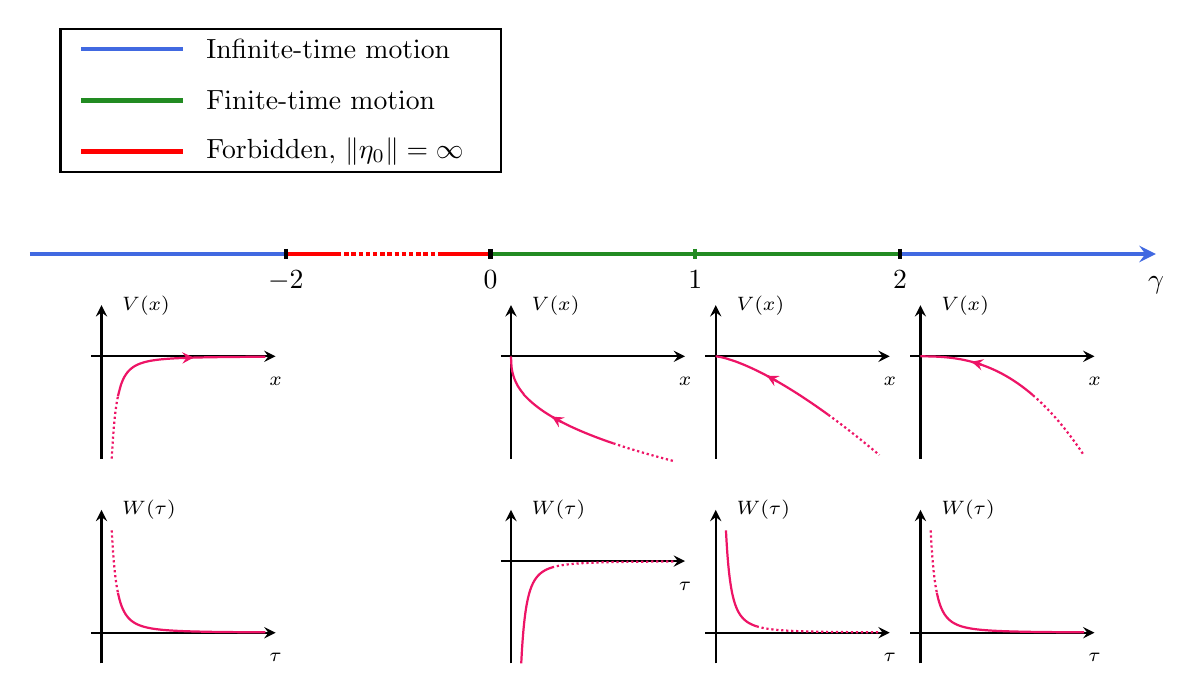
\begin{tikzpicture}[scale=1.3]
	\begin{scope}[ultra thick]
		% Axis
		\draw[RoyalBlue] (-0.5,0) -- (2,0);
		\draw[Red] (2,0) -- (2.5,0);
		\draw[densely dotted,Red] (2.5,0) -- (3.5,0);
		\draw[Red] (3.5,0) -- (4,0);
		\draw[ForestGreen] (4,0) -- (8,0);
		\draw[RoyalBlue, -stealth] (8,0) -- (10.5,0){};
		\draw (10.5,0) node[label={[label distance=0]below:$\gamma$}] {};
		\draw (2,0.05) -- (2,-0.05) node[label={[label distance=-4]below:$-2$}] {};
		\draw (4,0.05) -- (4,-0.05) node[label={[label distance=-4]below:$0$}] {};
		\draw[ForestGreen] (6,0.05) -- (6,-0.05);
		\draw (6,-0.05) node[label={[label distance=-4]below:$1$}] {};
		\draw (8,0.05) -- (8,-0.05) node[label={[label distance=-4]below:$2$}] {};
		% Legend
		\draw[thick] (-0.2, 2.2) -- (4.1, 2.2) -- (4.1, 0.8) -- (-0.2, 0.8) -- cycle;
		\draw[RoyalBlue] (0,2) -- (1,2);
		\draw (1,2) node[label={[label distance=0]right:Infinite-time motion}] {};
		\draw[ForestGreen] (0,1.5) -- (1,1.5);
		\draw (1,1.5) node[label={[label distance=0]right:Finite-time motion}] {};
		\draw[Red] (0,1) -- (1,1);
		\draw (1,1) node[label={[label distance=0]right:Forbidden, $\|\eta_0\| = \infty$}] {};
	\end{scope}
	\begin{scope}[thick]
		% V(x) plots
		\draw[-stealth] (0.1,-1) -- (1.9,-1) node[label={[label distance=0]below:$\scriptstyle x$}] {};
		\draw[-stealth] (0.2,-2) -- (0.2,-0.5) node[label={[label distance=0]right:$\scriptstyle V(x)$}] {};
		\draw[domain=0.3:0.36, smooth, variable=\x,WildStrawberry,densely dotted] plot ({\x}, {-0.01/(\x-0.2)^2-1});
		\draw[domain=0.36:1.1, smooth, variable=\x,WildStrawberry,-stealth] plot ({\x}, {-0.01/(\x-0.2)^2-1});
		\draw[domain=1:1.8, smooth, variable=\x,WildStrawberry] plot ({\x}, {-0.01/(\x-0.2)^2-1});
		\draw[-stealth] (4.1,-1) -- (5.9,-1) node[label={[label distance=0]below:$\scriptstyle x$}] {};
		\draw[-stealth] (4.2,-2) -- (4.2,-0.5) node[label={[label distance=0]right:$\scriptstyle V(x)$}] {};
		\draw[domain=4.2:4.7, smooth, variable=\x,WildStrawberry, samples=100] plot ({\x}, {-0.85*(\x-4.2)^0.4-1});
		\draw[domain=4.6:5.2, smooth, variable=\x,WildStrawberry, samples=100,stealth-] plot ({\x}, {-0.85*(\x-4.2)^0.4-1});
		\draw[domain=5.2:5.8, smooth, variable=\x,WildStrawberry, samples=100,densely dotted] plot ({\x}, {-0.85*(\x-4.2)^0.4-1});
		\draw[-stealth] (6.1,-1) -- (7.9,-1) node[label={[label distance=0]below:$\scriptstyle x$}] {};
		\draw[-stealth] (6.2,-2) -- (6.2,-0.5) node[label={[label distance=0]right:$\scriptstyle V(x)$}] {};
		\draw[domain=6.2:6.8, smooth, variable=\x,WildStrawberry, samples=100] plot ({\x}, {-0.5*(\x-6.2)^1.4-1});
		\draw[domain=6.7:7.3, smooth, variable=\x,WildStrawberry, samples=100,stealth-] plot ({\x}, {-0.5*(\x-6.2)^1.4-1});
		\draw[domain=7.3:7.8, smooth, variable=\x,WildStrawberry, samples=100,densely dotted] plot ({\x}, {-0.5*(\x-6.2)^1.4-1});
		\draw[-stealth] (8.1,-1) -- (9.9,-1) node[label={[label distance=0]below:$\scriptstyle x$}] {};
		\draw[-stealth] (8.2,-2) -- (8.2,-0.5) node[label={[label distance=0]right:$\scriptstyle V(x)$}] {};
		\draw[domain=8.2:8.8, smooth, variable=\x,WildStrawberry, samples=100] plot ({\x}, {-0.3*(\x-8.2)^2.5-1});
		\draw[domain=8.7:9.3, smooth, variable=\x,WildStrawberry, samples=100,stealth-] plot ({\x}, {-0.3*(\x-8.2)^2.5-1});
		\draw[domain=9.3:9.8, smooth, variable=\x,WildStrawberry, samples=100,densely dotted] plot ({\x}, {-0.3*(\x-8.2)^2.5-1});
		\draw[-stealth] (0.1,-3.7) -- (1.9,-3.7) node[label={[label distance=0]below:$\scriptstyle \tau$}] {};
		\draw[-stealth] (0.2,-4) -- (0.2,-2.5) node[label={[label distance=0]right:$\scriptstyle W(\tau)$}] {};
		\draw[domain=0.3:0.36, smooth, variable=\t,WildStrawberry,densely dotted] plot ({\t}, {0.01/(\t-0.2)^2-3.7});
		\draw[domain=0.36:1.8, smooth, variable=\t,WildStrawberry,samples=100] plot ({\t}, {0.01/(\t-0.2)^2-3.7});
		\draw[-stealth] (4.1,-3) -- (5.9,-3) node[label={[label distance=0]below:$\scriptstyle \tau$}] {};
		\draw[-stealth] (4.2,-4) -- (4.2,-2.5) node[label={[label distance=0]right:$\scriptstyle W(\tau)$}] {};
		\draw[domain=4.3:4.6, smooth, variable=\t,WildStrawberry,samples=150] plot ({\t}, {-0.01/(\t-4.2)^2-3});
		\draw[domain=4.6:5.8, smooth, variable=\t,WildStrawberry,densely dotted,samples=100] plot ({\t}, {-0.01/(\t-4.2)^2-3});	
		\draw[-stealth] (6.1,-3.7) -- (7.9,-3.7) node[label={[label distance=0]below:$\scriptstyle \tau$}] {};
		\draw[-stealth] (6.2,-4) -- (6.2,-2.5) node[label={[label distance=0]right:$\scriptstyle W(\tau)$}] {};
		\draw[domain=6.3:6.6, smooth, variable=\t,WildStrawberry,samples=150] plot ({\t}, {0.01/(\t-6.2)^2-3.7});
		\draw[domain=6.6:7.8, smooth, variable=\t,WildStrawberry,densely dotted,samples=100] plot ({\t}, {0.01/(\t-6.2)^2-3.7});
		\draw[-stealth] (8.1,-3.7) -- (9.9,-3.7) node[label={[label distance=0]below:$\scriptstyle \tau$}] {};
		\draw[-stealth] (8.2,-4) -- (8.2,-2.5) node[label={[label distance=0]right:$\scriptstyle W(\tau)$}] {};
		\draw[domain=8.3:8.36, smooth, variable=\t,WildStrawberry,densely dotted] plot ({\t}, {0.01/(\t-8.2)^2-3.7});
		\draw[domain=8.36:9.8, smooth, variable=\t,WildStrawberry,samples=100] plot ({\t}, {0.01/(\t-8.2)^2-3.7});			
	\end{scope}
\end{tikzpicture}

\end{document}